\documentclass[12pt]{article}
\usepackage{../../preamble2}

\title{UCLA Math Circle}
\author{James Toche (and family)}
\date{19 June 2020 \\(Last revision: \today)}

\begin{document}
\begin{minipage}{\textwidth}
\maketitle
\begin{abstract}
Notes on homework problems from the UCLA Math Circle Intermediate-2 for Summer Session 2020, July 19th. 
\end{abstract}
\end{minipage}

\section*{1a. Show by Induction that}
\begin{question}
  \begin{align*}
  1 + 2 + \ldots + n = \frac{n(n+1)}{2} \mathrlap{\qquad \forall n\geq 1}
  \end{align*}
\end{question}

This equality is an excellent introduction to the topic of \textbf{proof by induction}, because it can be proved in several other ways. Here are two standard proofs: a visual proof based on stacking and a proof based on rearranging terms. 
\subsubsection*{Just For Fun: A Proof by Stacking}
\begin{center}
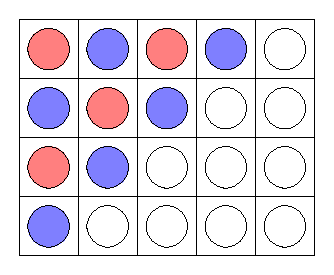
\includegraphics{tikz-matrix-nodes-circles-2}
\end{center}
Count the circles along the diagonal starting from the top-left corner, adding circles of the same color at each step (red, then blue, then red, then blue). The sequence is $1$ (for $n=1$), $3$ (for $n=2$), $6$ (for $n=3$), $10$ (for $n=4$). This last number is the sum of the first $4$ integers. Denote it $S_{4}$,
\begin{align*}
S_{4} = 1 + 2 + 3 + 4
\end{align*}
By symmetry, there are also $10$ white circles. Thus the total number of circles in the matrix is $2 \times S_{4} = 20$. But clearly, this is also the ``area'' of the rectangle $20=4\times5$ (height times width). The argument is general and therefore $2 S_{n} = n\times(n+1)$.  \qed

\subsubsection*{Just For Fun: A Proof by Rearrangement}
Rearrange the sum by reversing it:
\begin{align*}
S_{n}\quad & =\quad 1 \quad+\quad~~~~2 ~~~~\quad+\quad~~~~3 ~~~~\quad+\quad\ldots\quad+\quad(n-1) ~\quad+\quad~ n \\
      & =\quad n \quad+\quad (n-1) \quad+\quad (n-2) \quad+\quad\ldots\quad+\quad ~~~~2 ~~~~~\quad+\quad~ 1
\end{align*}
Consider the terms that are aligned vertically: The first two add up to $1+n$. The next two add up to $2+(n-1)=1+n$. Next, $3+(n-2)=1+n$. And so on. Thus the sum $2S_{n}$ is equal to a repeated sum of  $(1+n)$. How many times is the sum repeated? From the first line, exactly $n$ repetitions. And thus,
\begin{align*}
2 S_{n} 
  & = \underbrace{(1+n) \quad+\quad \ldots \quad+\quad (1+n)}_{\text{$n$ times}} \\
  & = (1+n) \times n \quad \qed
\end{align*}
\subsubsection*{Proof by Induction}
\begin{align*}
P(n): \quad
 S_{n} = 1 + 2 + \ldots + n = \frac{n(n+1)}{2}
\end{align*} 
To prove $P(n)$ true for all $n\geq1$, we prove the two statements:
\begin{align*}
\begin{cases}
& P(n) ~\text{true for $n=1$} ~\text{(Base Case)}\\
& \text{if}~P(n)~\text{is true for some $n$, then}~ P(n+1)~\text{is also true} ~\text{(Induction Step)}
\end{cases}
\end{align*}
These two statements together imply: $P(n)$ true for all $n\geq1$.

An equivalent, more concise way of writing the two parts of a proof by induction is:
\begin{align*}
\begin{cases}
& P(1) ~\texttt{true} \\
& P(n) \implies P(n+1)
\end{cases}
\end{align*}
The two-step procedure above is a template for most proofs by induction. 

\underline{Base Case:} 

Substitute $n$ for $1$:
\begin{align*}
P(1): \quad
  1 = \frac{1 \times (1+1)}{2} \mathrlap{\qquad \cmark}
\end{align*}
\underline{Induction Step:} 

Start with the left-hand side of $P(n+1)$ and substitute $P(n)$ to get the right-hand side of $P(n+1)$, where
\begin{align*}
P(n+1): \quad
 1 + 2 + \ldots + n + (n+1) = \frac{(n+1)(n+2)}{2}
\end{align*}
From the left-hand side of $P(n+1)$:
\begin{alignat*}{4}
\texttt{lhs} \quad
 &=& \quad & \underbrace{1 + 2 + \ldots + n} \quad &+\quad (n+1) \\
 &=& \quad & \quad \frac{n(n+1)}{2} \quad &+\quad (n+1)  \\
 &=& \quad & \frac{n(n+1)+2(n+1)}{2} \\
 &=& \quad & \frac{(n+1)(n+2)}{2} \\
 &=& \quad & \texttt{rhs} & \qed
\end{alignat*}


\clearpage

\section*{1b. Show by Induction that}
\begin{question}
  \begin{align*}
  1 + 3 + \ldots + (2n-1) = n^{2} \mathrlap{\qquad \forall n\geq 1}
  \end{align*}
\end{question}
Let $P(n)$ denote	the equality for \textit{some} fixed value $n\in\mathbb{N}$. We have:
\begin{align*}
P(n+1): \quad
  1 + 3 + \ldots + (2n-1) + (2n+1) = (n+1)^{2}
\end{align*}
\underline{Base Case:}
\begin{align*}
P(1): \quad
  1 = 1^{2} \mathrlap{\qquad \cmark}
\end{align*}
\underline{Induction Step:}
\begin{alignat*}{4}
\texttt{lhs} \quad
 &=& \quad &\underbrace{1 + 3 + \ldots + (2n-1)} \quad &+ \quad (2n+1) \\
 &=& \quad &\makebox[10em]{$n^{2}$} &+ \quad (2n+1)  \\
 &=& \quad & n^{2}+ 2n + 1 \\
 &=& \quad & (n + 1)^{2} \\
 &=& \quad & \texttt{rhs} & \qed 
\end{alignat*}



\section*{1c. Show by Induction that}
\begin{question}
  \begin{align*}
  2 + 5 + \ldots + (3n-1) = \frac{3n^{2}+n}{2} \mathrlap{\qquad \forall n\geq 1}
  \end{align*}
\end{question}
Let $P(n)$ denote	the equality for \textit{some} fixed value $n\in\mathbb{N}$. We have:
\begin{align*}
P(n+1): \quad
  2 + 5 + \ldots + (3n-1) + (3n+2) = \frac{3(n+1)^{2}+(n+1)}{2}
\end{align*}
\underline{Base Case:}
\begin{align*}
P(1): \quad
  2 = \frac{3\cdot1^{2}+1}{2} \mathrlap{\qquad \cmark}
\end{align*}
\underline{Induction Step:}
\begin{alignat*}{4}
\texttt{lhs} \quad
 &=& \quad &\underbrace{2 + 5 + \ldots + (3n-1)} \quad &+ \quad (3n+2) \\
 &=& \quad &\makebox[10em]{$\dfrac{3n^{2}+n}{2}$} &+ \quad (3n+2)  \\
 &=& \quad & \frac{3n^{2}+7n+4}{2}
\end{alignat*}
While we could factorize the above expression to make $(n+1)$ appear, it is easier to expand the right-hand side of $P(n+1)$ and show that it is equal to the left-hand side. Thus,
\begin{alignat*}{4}
\texttt{rhs} \quad
 &=& \quad & \frac{3(n+1)^{2}+(n+1)}{2} \\
 &=& \quad & \frac{3(n^{2}+2n+1)+n+1}{2} \\
 &=& \quad & \frac{3n^{2}+7n+4}{2} \\
 &=& \quad & \texttt{lhs} & \qed 
\end{alignat*}



\section*{1d. Show by Induction that}
\begin{question}
  \begin{align*}
  1 + 2^{2} + \dots + n^{2} = \frac{n(n+1)(2n+1)}{6} \mathrlap{\qquad \forall n\geq 1}
  \end{align*}
\end{question}
Let $P(n)$ denote	the equality for \textit{some} fixed value $n\in\mathbb{N}$. We have:
\begin{align*}
P(n+1): \quad
  1 + 2^{2} + \ldots + n^{2} + (n+1)^{2} = \frac{(n+1)(n+2)(2n+3)}{6}
\end{align*}
\underline{Base Case:}
\begin{align*}
P(1): \quad
  1 = \frac{1\cdot(1+1)(2\cdot1+1)}{6} \mathrlap{\qquad \cmark}
\end{align*}
\underline{Induction Step:}
\begin{alignat*}{4}
\texttt{lhs} \quad
 &=& \quad &\underbrace{1 + 2^{2} +\dots+ n^{2}} \quad &+ \quad (n+1)^{2} \\
 &=& \quad &\makebox[8em]{$\dfrac{n(n+1)(2n+1)}{6}$} &+ \quad (n+1)^{2} \\
 &=& \quad & \frac{n(n+1)(2n+1)+6(n+1)^{2}}{6} \\
 &=& \quad & \frac{(n+1)\,[n(2n+1)+6(n+1)]}{6} \\
 &=& \quad & \frac{(n+1)(2n^{2}+7n+6)}{6} 
\end{alignat*}
While we could factorize the above expression to make $(n+2)(2n+3)$ appear, it is easier to expand the right-hand side of $P(n+1)$ and show that it is equal to the left-hand side. Thus,
\begin{alignat*}{4}
\texttt{rhs} \quad
 &=& \quad & \frac{(n+1)(n+2)(2n+3)}{6} \\
 &=& \quad & \frac{(n+1)(2n^{2}+7n+6)}{6} \\
 &=& \quad & \texttt{lhs} & \qed 
\end{alignat*}


\clearpage
\section*{2. Divisibility by Induction}
\begin{question}
Prove that the number $11\ldots11$ consisting of $243$ ones is divisible by $243$. Prove the generalization: for any positive integer $n$, the number consisting of $3^{n}$ ones is divisible by $3^{n}$.
\end{question}

The general statement is:
\begin{align*}
\underbrace{~11\ldots11~}_{\makebox[5pt]{$3^{n}$}~~\text{times}} 
 \quad=\quad 3^{n} \times m \mathrlap{\quad \text{for some}~ m\in\mathbb{N}}
\end{align*}
Special cases that are easy to check:
\begin{align*}
& P(1): \quad 111 \quad=\quad 3 \times 37 \\
& P(2): \quad 111,111,111 \quad=\quad 3^{2} \times 12345679
\end{align*}
To prove that $111,111,111$ is divisible by $9$ using divisibility rules, first note that:
\begin{align*}
111,000,000 & \\
+~111,000 &\\
+~111 & \\[-3\jot]
\rule{12ex}{0.4pt} \\[-1\jot]
111,111,111 & 
\end{align*}
so that 
\begin{align*}
111,111,111 
 & \quad=\quad 111 \cdot 10^{6} + 111 \cdot 10^{3} + 111 \cdot 10^{0} \\
 & \quad=\quad 111 \cdot (10^{6}+10^{3}+1)
\end{align*}
Because $111$ is a multiple of $3$ (its digits add up to $3$) and $10^{6}+10^{3}+1$ is a multiple of $3$ (its digits also add up to $3$), it follows that $111,111,111$ is a multiple of $3\times3=9$.

The above proof can be generalized. Let $a(n)$ denote the number:
\begin{align*}
P(n): \quad a(n) ~=~ \underbrace{111,111,111}_{3^{n}} \quad\text{is divisible by}~3^{n}
\end{align*}
The next number $a(n+1)$ may be written as:
\begin{align*}
a(n+1) 
 & ~=~ \underbrace{111,111,111}_{3^{n+1}} \\
 & ~=~ \underbrace{a(n) a(n) a(n)}_{3~\text{copies of}~a(n)} \\
 & ~=~ a(n) \cdot 10^{x} + a(n) \cdot 10^{y} + a(n) \\
 & ~=~ a(n) \cdot (10^{x} + 10^{y} + 1)
\end{align*}
where $y=3^{n}$ and $x=2y$ (but the exact values do not matter for the proof). By $P(n)$, we have $a(n)$ a multiple of $3^{n}$ and by the divisible rule, we have $10^{x}+10^{y}+1$ a multiple of $3$, and therefore $P(n+1)$ is true:
\begin{align*}
P(n+1): \quad a(n+1) ~=~ \underbrace{111,111,111}_{3^{n+1}} \quad\text{is divisible by}~3^{n+1} \qquad \qed
\end{align*}


\clearpage
\section*{3. Divisibility by Induction}
\begin{question}
Show that $n^{3}+2n$ is divisible by $3$ for all positive integers $n$. 
\end{question}

Suppose the proposition $P(n)$ is true for some $n\in\mathbb{N}$: 
\begin{align*}
P(n): \quad n^{3}+2n = 3m, ~\text{for some}~m\in\mathbb{N}
\end{align*}
\underline{Base Case:}
\begin{align*}
P(1): \quad
  1^{3} + 2\cdot 1 = 3 \cdot 1 \mathrlap{\qquad \cmark}
\end{align*}
\underline{Induction Step:}
\begin{align*}
P(n+1): \quad
  (n+1)^{3}+2(n+1) = 3l, ~\text{for some}~l\in\mathbb{N}
\end{align*}
We start from the left-hand side of $P(n+1)$,
\begin{align*}
\texttt{lhs} \quad
& = \quad (n+1)^{3} + 2(n+1) \\
& = \quad n^{3} + 3n^{2} + 3n + 1 + 2n + 2 \\
& = \quad \underbrace{~n^{3} + 2n~} \quad+\quad 3(n^{2}+n+1) \\
& = \quad \makebox[4em]{$3m$} \quad+\quad 3(n^{2}+n+1) \\
& = \quad 3 (m+n^{2}+n+1) \\
& = \quad 3l, ~\text{where}~l\in\mathbb{N}~\text{because}~m,n,n^{2},1\in\mathbb{N} \\
& = \quad \texttt{rhs}
\end{align*}
\underline{Conclusion:}

Since $P(n)\implies P(n+1)$ and $P(1)$ true, it follows that $P(n)$ true for all $n\geq1$.

\clearpage
\section*{4a. Inequality by Induction}
\begin{question}
Show that for any positive integer $n$, we have $2^{n}>n$.
\end{question}

Suppose the proposition $P(n)$ is true for some $n\in\mathbb{N}$: 
\begin{align*}
P(n): \quad 
  2^{n} > n
\end{align*}
\underline{Base Case:}
\begin{align*}
P(1): \quad
  2^{1} > 1 \mathrlap{\qquad \cmark}
\end{align*}
\underline{Induction Step:}
\begin{align*}
P(n+1): \quad 
  2^{n+1} > n+1
\end{align*}
We start from the left-hand side of $P(n+1)$:
\begin{align*}
\texttt{lhs} \quad
& = \quad 2^{n+1} \\
& = \quad 2 \cdot \underbrace{~~2^{n}~~}_{\makebox[2em]{$>n$}} \\
& > \quad 2 n \\
& > \quad n + n \\
& > \quad n + 1 \quad=\quad \texttt{rhs}
\end{align*}
where the last inequality follows from $n \geq 1$.

\underline{Conclusion:}

Since $P(n)\implies P(n+1)$ and $P(1)$ true, it follows that $P(n)$ true for all $n\geq1$.



\clearpage
\section*{4b. Inequality by Induction}
\begin{question}
Find all positive integers $n$ such that $2^{n}>n^{2}$. Prove the result.
\end{question}

We tabulate the first few cases:

\begin{center}
\renewcommand{\arraystretch}{1.5}
\newcolumntype{C}[1]{>{\centering\arraybackslash}p{#1}} % centered 'p' col.
\begin{tabular}{*{4}{C{0.17\linewidth}}}
    \hline
    $n$  &  $2^{n}$ &  $n^{2}$ & $2^{n}>n^{2}$ \\
    \hline
    $0$  &  $1$     &  $0$     & true \\
    $1$  &  $2$     &  $1$     & true \\
    $2$  &  $4$     &  $4$     & false \\
    $3$  &  $8$     &  $9$     & false \\
    $4$  &  $16$    &  $16$    & false \\
    $5$  &  $32$    &  $25$    & true \\
    $6$  &  $64$    &  $36$    & true \\
    $7$  &  $128$   &  $49$    & true \\
    \hline
    \end{tabular}
\end{center}

Our hypothesis is that the inequality holds for $n\geq 5$. This hypothesis follows by inspecting the graphs of $2^{n}$ and $n^{2}$. 
We prove the hypothesis by induction. Suppose the proposition is true for some $n\in\mathbb{N}$:
\begin{align*}
P(n): \quad 
  2^{n} > n^{2}
\end{align*}
\underline{Base Case:}
\begin{align*}
P(5): \quad
  2^{5} > 5^{2} \mathrlap{\qquad \cmark}
\end{align*}
\underline{Induction Step:}
\begin{align*}
P(n+1): \quad 
  2^{n+1} > (n+1)^{2}
\end{align*}
We start from the left-hand side of $P(n+1)$:
\begin{align*}
\texttt{lhs} \quad
& = \quad 2^{n+1} \\
& = \quad 2 \cdot \underbrace{~~2^{n}~~}_{>n^{2}} \\
& > \quad 2 n^{2} = \quad n^{2} + n^{2}
\end{align*}
Now consider the right-hand side of $P(n+1)$:
\begin{align*}
\texttt{rhs} \quad
& = \quad (n+1)^{2} \\
& = \quad n^{2} + 2n + 1
\end{align*}
Thus, $2^{n+1}>(n+1)^{2}$ if $n^{2}>2n+1$. This is true for $n\geq 5$ because it is true for $n=5$ and $n^{2}$ increases faster than $2n+1$ as $n$ is increased.

\underline{Conclusion:}

Since $P(n)\implies P(n+1)$ and $P(5)$ true, it follows that $P(n)$ true for all $n\geq5$.


\clearpage
\section*{5. Lines \& Regions}
\begin{question}
Suppose there are $n$ lines drawn in the plane such that no two lines are parallel and no three lines intersect at the same point. Find a closed formula for the number of regions that the lines split into.
\end{question}

For small values of $n$, it is easy to sketch intersecting lines and count regions. Let $n$ denote the number of lines and $r$ the number regions. We have:
\begin{center}
\renewcommand{\arraystretch}{1.5}
\newcolumntype{C}[1]{>{\centering\arraybackslash}p{#1}} % centered 'p' col.
\begin{tabular}{*{2}{C{0.12\linewidth}}}
    \toprule
    n  &  r \\
    \midrule
    $0$  &  $1$ \\
    $1$  &  $2$ \\
    $2$  &  $4$ \\
    $3$  &  $7$ \\
    $4$  &  $11$ \\
    \bottomrule
    \end{tabular}
\end{center}
The case $n=0$ is obvious: with no lines crossing the plane, there is one region --- the entire plane. 

The case $n=1$ is equally obvious: a single line divides the plane into two regions, each being a half-plane. 

The case $n=2$ is easy to explain: At the intersection of the two lines, there are four angles that sum to $360^{\circ}$, and each angle defines a region. 

The case $n=3$ can be explained by extending the previous idea: The intersection of the three lines forms a triangle. This triangle defines one region. Now move the lines such as to shrink the triangle to a single point. The resulting figure has three lines intersecting at a single point (see figure below). These lines define $6$ regions, for a total of $7$ regions when the triangle is included. 
\begin{center}
\begin{tikzpicture}
  \draw [black, thick] (0.4,0.4) -- +(0:1.4) -- +(180:2.2); 
  \draw [black, thick] (-0.2:-0.2) -- +(120:2) -- +(300:2); 
  \draw [black, thick] (0.2:0.2) -- +(240:2) -- +(60:2); 
\begin{scope}[xshift=8cm]
  \draw [black, thick] (0:0) -- +(0:2) -- +(180:2); 
  \draw [black, thick] (0:0) -- +(120:2) -- +(300:2); 
  \draw [black, thick] (0:0) -- +(240:2) -- +(60:2); 
\end{scope}
\end{tikzpicture}
\end{center}
The case $n=4$ can be understood by considering what happens when a line is added to the previous case. The fourth line intersects the other three lines at $3$ points, and so goes through $4$ ``existing'' regions, dividing each into two parts, thus adding $4$ ``new'' regions, $7+4=11$. 

In general, the $n$th line intersects with $n-1$ lines, creating $n$ news regions. This suggests a method for calculating the number of regions based on the previous value:
\begin{align*}
r(n) = r(n-1) + n
\end{align*}
This is a linear recurrence. A linear recurrence admits a unique solution, which may be found, for instance, by repeated substitution. 
\begin{align*}
  r(n) & = r(n-1) + n \\
r(n-1) & = r(n-2) + (n-1) \\
r(n-2) & = r(n-3) + (n-2) \\
       & \vdotswithin{=} \\
  r(3) & = r(2) + 3 \\
  r(2) & = r(1) + 2 \\
  r(1) & = r(0) + 1 
\end{align*}
Adding these equalities column-wise gives:
\begin{align*}
r(n) = n + (n-1) + (n-2) + \ldots + 3 + 2 + 1 + r(0)
\end{align*}
where $r(0)=1$ (as noted in the table above). Thus,
\begin{align*}
r(n) = (1 + 2 + 3 + \ldots + n) + 1 
\end{align*}
In words, the number of regions delimited by the intersection of $n$ lines that intersect at $n-1$ distinct points is equal to one plus the sum of the integers up to $n$. There is, of course, a famous formula for the sum of the first $n$ integers: 
\begin{align*}
1 + 2 + 3 + \ldots + n = \frac{n(n+1)}{2}
\end{align*}
Substituting into the formula for $r(n)$ gives:
\begin{align*}
r(n) 
 & = \frac{n(n+1)}{2} + 1 \\
 & = \frac{n^2 + n + 2}{2}
\end{align*}

For peace of mind, you may check that the formula generates the values computed in the table above:
\begin{align*}
r(0) & = \frac{0^2 + 0 + 2}{2} = \frac{2}{2} = 1 \\
r(1) & = \frac{1^2 + 1 + 2}{2} = \frac{4}{2} = 2 \\
r(2) & = \frac{2^2 + 2 + 2}{2} = \frac{8}{2} = 4 \\
r(3) & = \frac{3^2 + 3 + 2}{2} = \frac{14}{2} = 7 \\
r(4) & = \frac{4^2 + 4 + 2}{2} = \frac{22}{2} = 11
\end{align*}


\end{document}
